\documentclass[dvipdfmx]{ehis}
\usepackage{graphicx}

\usepackage{amsmath,amssymb,amsfonts}
\usepackage{algorithmic}
\usepackage{textcomp}
\usepackage{xcolor}
\usepackage{url}
\usepackage{booktabs}
\usepackage[caption=false]{subfig}
\usepackage{multirow}
\usepackage{algorithm}
\usepackage{algorithmic}
\usepackage{listings}
\lstdefinelanguage{JavaScript}{
  keywords={const, let, var, function, return, if, else, for, while, switch, case, break, try, catch, finally, window, camerala_logger},
  sensitive=true,
  comment=[l]{//},
  morecomment=[s]{/*}{*/},
  morestring=[b]\",
  morestring=[b]\'
}
\lstdefinelanguage{csv}{
  morecomment=[l]{\#},
}

\newcommand{\etal}{\textit{et al.}}
\newcommand{\ie}{\textit{i.e.}}
\newcommand{\eg}{\textit{e.g.}}

\etitle{Camerala: A Local-First Browser-Native Framework for Remote Psychophysiological Task Sensing}

\eauthor{
Kotaro Furukawa\thanks{College of Transdisciplinary Sciences for Innovation, Kanazawa University, Japan}
}

\YEAR{}
\VOL{}
\NO{}
\TYPE{}


\lstset{
  basicstyle=\ttfamily\scriptsize,
  breaklines=true,
  columns=fullflexible,
  keepspaces=true
}
\makeatletter
\def\@oddhead{}
\def\@evenhead{}
\def\ps@vr{
 \def\@oddhead{}
 \def\@evenhead{}
}
\def\ps@his{
 \def\@oddhead{}
 \def\@evenhead{}
}
\makeatother

\begin{document}

\begin{abstract}
Camerala is a local-first, browser-native framework for remote psychological and psychophysiological task experiments.
It synchronizes task events with face-image-derived feature records and exports local CSV/ZIP files without transmitting or storing raw facial video.
In an exploratory N=1 author-participant deployment, ten sessions were conducted in laboratory and home settings, yielding 600 trials in total.
After applying a reaction-time criterion of 100--1500 ms, 541/600 trials remained for descriptive analysis.
The exported logs contained timestamped task events and reproducible face-image-derived fields.
Differences between laboratory and home exported records are reported as deployment-context differences in face-derived and sensor-derived records, not as evidence of psychological, physiological, cognitive, motivational, or rPPG-accuracy effects.
\end{abstract}

\begin{keyword}
Browser-Native Sensing, Remote Photoplethysmography, FaceMesh, Local-First Logging, Task-Aligned Measurement, Laboratory and Home Settings
\end{keyword}

\maketitle

% =================================================================================
% SECTION 1: INTRODUCTION
% =================================================================================
\section{Introduction}

The intended use case of Camerala is a browser-based remote psychological/psychophysiological task experiment conducted in laboratory and home settings.
In this use case, the participant sits in front of a laptop, views task stimuli, and responds by key press.
Camerala is not intended for continuous physiological sensing during ordinary daily activities.
Rather, Camerala supports task-synchronized acquisition of face-derived records while reducing the need to transmit or retain privacy-sensitive raw facial video.
Even in this task-based experiment, deployment outside a controlled laboratory introduces practical difficulties for human-interface research, including heterogeneous illumination, camera placement, posture, browser timing, and local data handling.

Many video-based physiological measurement pipelines rely on raw video recording or server-side processing.
Such approaches can be difficult to deploy in private spaces because raw facial video is privacy-sensitive and may be identifiable.
A local-first browser architecture offers an architectural privacy advantage: raw frames can be processed on the client device, while only extracted features, task events, and quality indicators are stored.
This does not constitute a dedicated privacy-preserving algorithm; rather, it is a system-design choice that reduces the need to transmit or retain raw video.

Real-time processing is not treated as the only technically possible architecture.
Local video recording followed by offline processing could preserve timestamps if implemented carefully.
However, the intended use case of Camerala is a browser-based remote psychological/psychophysiological task experiment conducted in laboratory and home settings, where retaining identifiable facial video for later analysis can itself be a privacy and acceptability burden.
Camerala therefore extracts face-image-derived records during task execution and stores only task events, exported feature fields, and auxiliary context fields, without raw facial video persistence.
In this sense, real-time browser-side processing is used to support feature-only local logging and timestamp alignment within the same client-side runtime, rather than to claim more accurate physiological estimates or online task adaptation.

To address this deployment scenario, we present \textbf{Camerala}, a browser-native framework for task-aligned physiological feature logging in remote task experiments.

\subsection{Research Questions}
The exploratory Research Questions (RQs) focus on task-synchronized face-derived records and descriptive sensor-derived observations under the tested configuration:
\begin{itemize}
    \item \textbf{RQ1:} In the intended remote psychological/psychophysiological task use case, do Camerala's task-synchronized face-derived records, including rPPG-oriented ROI values, satisfy the operational criteria for descriptive analysis: trial-level reaction times within 100--1500 ms and exported-window-level landmark availability of \texttt{mean\_quality} $\geq$ 0.8 under the tested configuration?
    \item \textbf{RQ2:} What kinds of between-environment differences are observable in the physiological signals collected through such a deployment?
\end{itemize}

For RQ1, we evaluated the exported records using operational criteria at the trial and exported-window levels.
At the trial level, trials were retained for descriptive analysis when reaction times fell within 100--1500 ms.
At the exported-window level, landmark availability was evaluated using \texttt{mean\_quality}, the mean of the binary landmark-availability flag within each 10-s window; exported windows with \texttt{mean\_quality} $\geq$ 0.8 were treated as satisfying the operational landmark-availability criterion.
This criterion describes the exported frame/window records and should not be interpreted as face-detection availability across all camera frames.
We also examined whether the exported records contained reproducible face-derived fields, including rPPG-oriented ROI values, motion estimates, and a frame-to-frame green-channel brightness-change indicator.
In RQ2, the term ``physiological signals'' is used operationally to refer to task-synchronized face-derived and sensor-derived exported records, including rPPG-oriented ROI values and related exported fields.
These records are not treated as validated physiological-state measurements.
The present design was not able to determine whether laboratory/home differences reflected psychological state, physiological state, lighting, screen light, posture, camera geometry, the measurement pipeline, task timing, participant state, or their mixture.
Therefore, laboratory/home differences were interpreted as deployment-context differences rather than psychological, cognitive, motivational, or physiological effects.
These analyses are intended only to describe operational completion and exported-record differences under the tested configuration; they do not demonstrate general deployability across users, devices, or environments.

\subsection{Contributions}
In this paper, we focus on system integration and conservative deployment observations. The contributions are:

\begin{enumerate}
    \item \textbf{Local-first browser-native system-integration implementation}: An implementation for remote psychological and psychophysiological task experiments that combines task execution, face-derived feature extraction, timestamp alignment, and local persistence within one browser runtime.
    \item \textbf{Task-synchronized feature logging pipeline}: A logging pipeline that records task events, rPPG-oriented ROI values, FaceMesh-derived motion estimates, operational landmark-availability ratios, and frame-derived brightness-change indicators without raw facial video persistence.
    \item \textbf{Exploratory deployment under limited conditions}: An N=1 author-participant deployment showing that, under the tested configuration, the exported records satisfied the specified reaction-time and landmark-availability criteria for descriptive analysis.
\end{enumerate}

The remainder of this paper is organized as follows.
Section II reviews related work in rPPG, web/edge physiological sensing, and task-measurement platforms.
Section III describes the Camerala system architecture.
Section IV describes the browser-based task deployment and reporting details.
Section V presents descriptive observations.
Section VI discusses design requirements and safeguards for future deployments, and Section VII concludes.

% =================================================================================
% SECTION 2: RELATED WORK
% =================================================================================
\section{Related Work}

\subsection{Remote Physiological Measurement and rPPG}
Remote photoplethysmography (rPPG) estimates pulse-related color changes from facial video.
Classic approaches include ambient-light remote plethysmographic imaging and blind-source video methods \cite{verkruysse2008,poh_ica}, while more recent work includes deep-learning-based estimators \cite{deepphys}.
These studies show that camera-based and webcam-based rPPG functionality already exists.
They also show that uncontrolled capture conditions, implementation choices, and evaluation pipelines are important factors in remote heart-rate imaging.
Accordingly, Camerala does not claim to introduce a new rPPG estimator or to solve rPPG degradation under uncontrolled conditions.
It records rPPG-oriented ROI values and exported indicators so that task-aligned records can be inspected descriptively.

\subsection{Browser-Based, Web-Deployable, Edge-Based, and Privacy-Oriented rPPG Systems}
Several closely related prior studies and systems are directly relevant to Camerala's positioning.
Ayesha \etal\ proposed a web application for experimenting with and validating remote measurement of vital signs \cite{ayesha_web_vital}.
LabVanced provides remote heart-rate detection/rPPG functionality within an online experiment platform \cite{labvanced_rppg}.
FacePhys-Demo demonstrates browser-based rPPG monitoring with local inference in a public web demo/repository \cite{facephys_demo}.
RhythmEdge addresses contactless heart-rate estimation on edge devices \cite{rhythmedge}.
Gupta and Etemad investigated privacy-preserving remote heart-rate estimation from facial videos \cite{gupta_privacy}.
Di Lernia \etal\ evaluated rPPG via online webcams under uncontrolled conditions \cite{di_lernia_rppg_wild}.
Together, these related studies and public systems indicate that browser-based, web-deployable, edge-based, and privacy-oriented rPPG have already been explored.
Camerala therefore does not claim novelty in browser-based rPPG functionality, local rPPG processing, edge-oriented heart-rate estimation, or privacy preservation as an algorithm.
Instead, Camerala is positioned as a system-integration implementation for remote psychological and psychophysiological task experiments: it combines browser-based task execution, face-derived feature extraction, task-event/frame-record timestamp alignment, operational landmark-availability checking, and local CSV/ZIP persistence without raw facial video retention within one browser runtime.

\subsection{Task Measurement and Physiological Data Collection Platforms}
Well-established web experiment libraries and experiment runtimes, such as jsPsych \cite{jspsych_joss} and PsychoPy/PsychoJS/Pavlovia \cite{psychopy2}, support browser-based task execution and online experiments.
However, they do not generally provide an integrated webcam-derived physiological feature pipeline, task-sensing synchronization, and local-first feature logging as a single browser runtime.
Conversely, cloud analytics APIs can provide rich video-based analysis but often require transmitting video streams away from the participant's device.
Table \ref{tab:related_work} maps this design trade-off space.

\begin{table*}[t]
    \begin{center}
    \caption{Design Trade-off Mapping of Data Collection Platforms}
\label{tab:related_work}
\scriptsize
\setlength{\tabcolsep}{2pt}
\begin{tabular}{p{0.20\textwidth}p{0.14\textwidth}p{0.15\textwidth}p{0.14\textwidth}p{0.11\textwidth}p{0.11\textwidth}}
\toprule
\textbf{System / Platform} & \textbf{On-device video processing} & \textbf{Task-sensing synchronization} & \textbf{Local-first persistence} & \textbf{Raw video export} & \textbf{Typical use} \\
\midrule
Web experiment libraries & N/A (task only) & Partial & Depends on setup & N/A & Behavioral tasks \\
Experiment runtimes & Depends on deployment & Yes for task events & Depends on setup & Depends & Lab/online experiments \\
Browser or web rPPG systems & Often possible & Usually not task-centered & Varies & Varies & Vital-sign estimation \\
Cloud sensing APIs & No & Low or asynchronous & No & Often required & Video analytics \\
\textbf{Camerala} & Client-side feature extraction & Task events and frame features in one runtime & Local ZIP export of logs & Not used by Camerala & Remote task studies \\
\bottomrule
\end{tabular}
\vspace{1mm}

\scriptsize{\textit{Note: The table summarizes design emphasis rather than categorical superiority. Capabilities depend on implementation and deployment configuration.}}
\end{center}
\end{table*}

We structure the initial evaluation as a single-case exploratory deployment.
The deployment is not intended to estimate population-level psychological or physiological effects.
Instead, it documents whether the integrated browser runtime can complete the planned browser-based task logging procedure and what measurement-quality differences are observed in the tested laboratory and home contexts.

% =================================================================================
% SECTION 3: SYSTEM ARCHITECTURE
% =================================================================================
\section{System Architecture: Camerala}
\textbf{Camerala} (derived from "Camera" + "Laboratory") is positioned as a local-first, browser-native research implementation for remote psychological and psychophysiological task experiments.
Its contribution is not browser-based rPPG, local rPPG processing, or privacy preservation as an algorithm.
Rather, it integrates task execution, face-derived feature extraction, task-event/frame-record timestamp alignment, operational landmark-availability checking, and local CSV/ZIP persistence without raw facial video retention within one browser runtime.
Although the deployment in this paper used one Gabor-orientation task, the runtime separates task logic from the sensing pipeline so that other task procedures can be implemented without changing the feature-extraction loop.

\begin{figure}[t]
    \begin{center}
    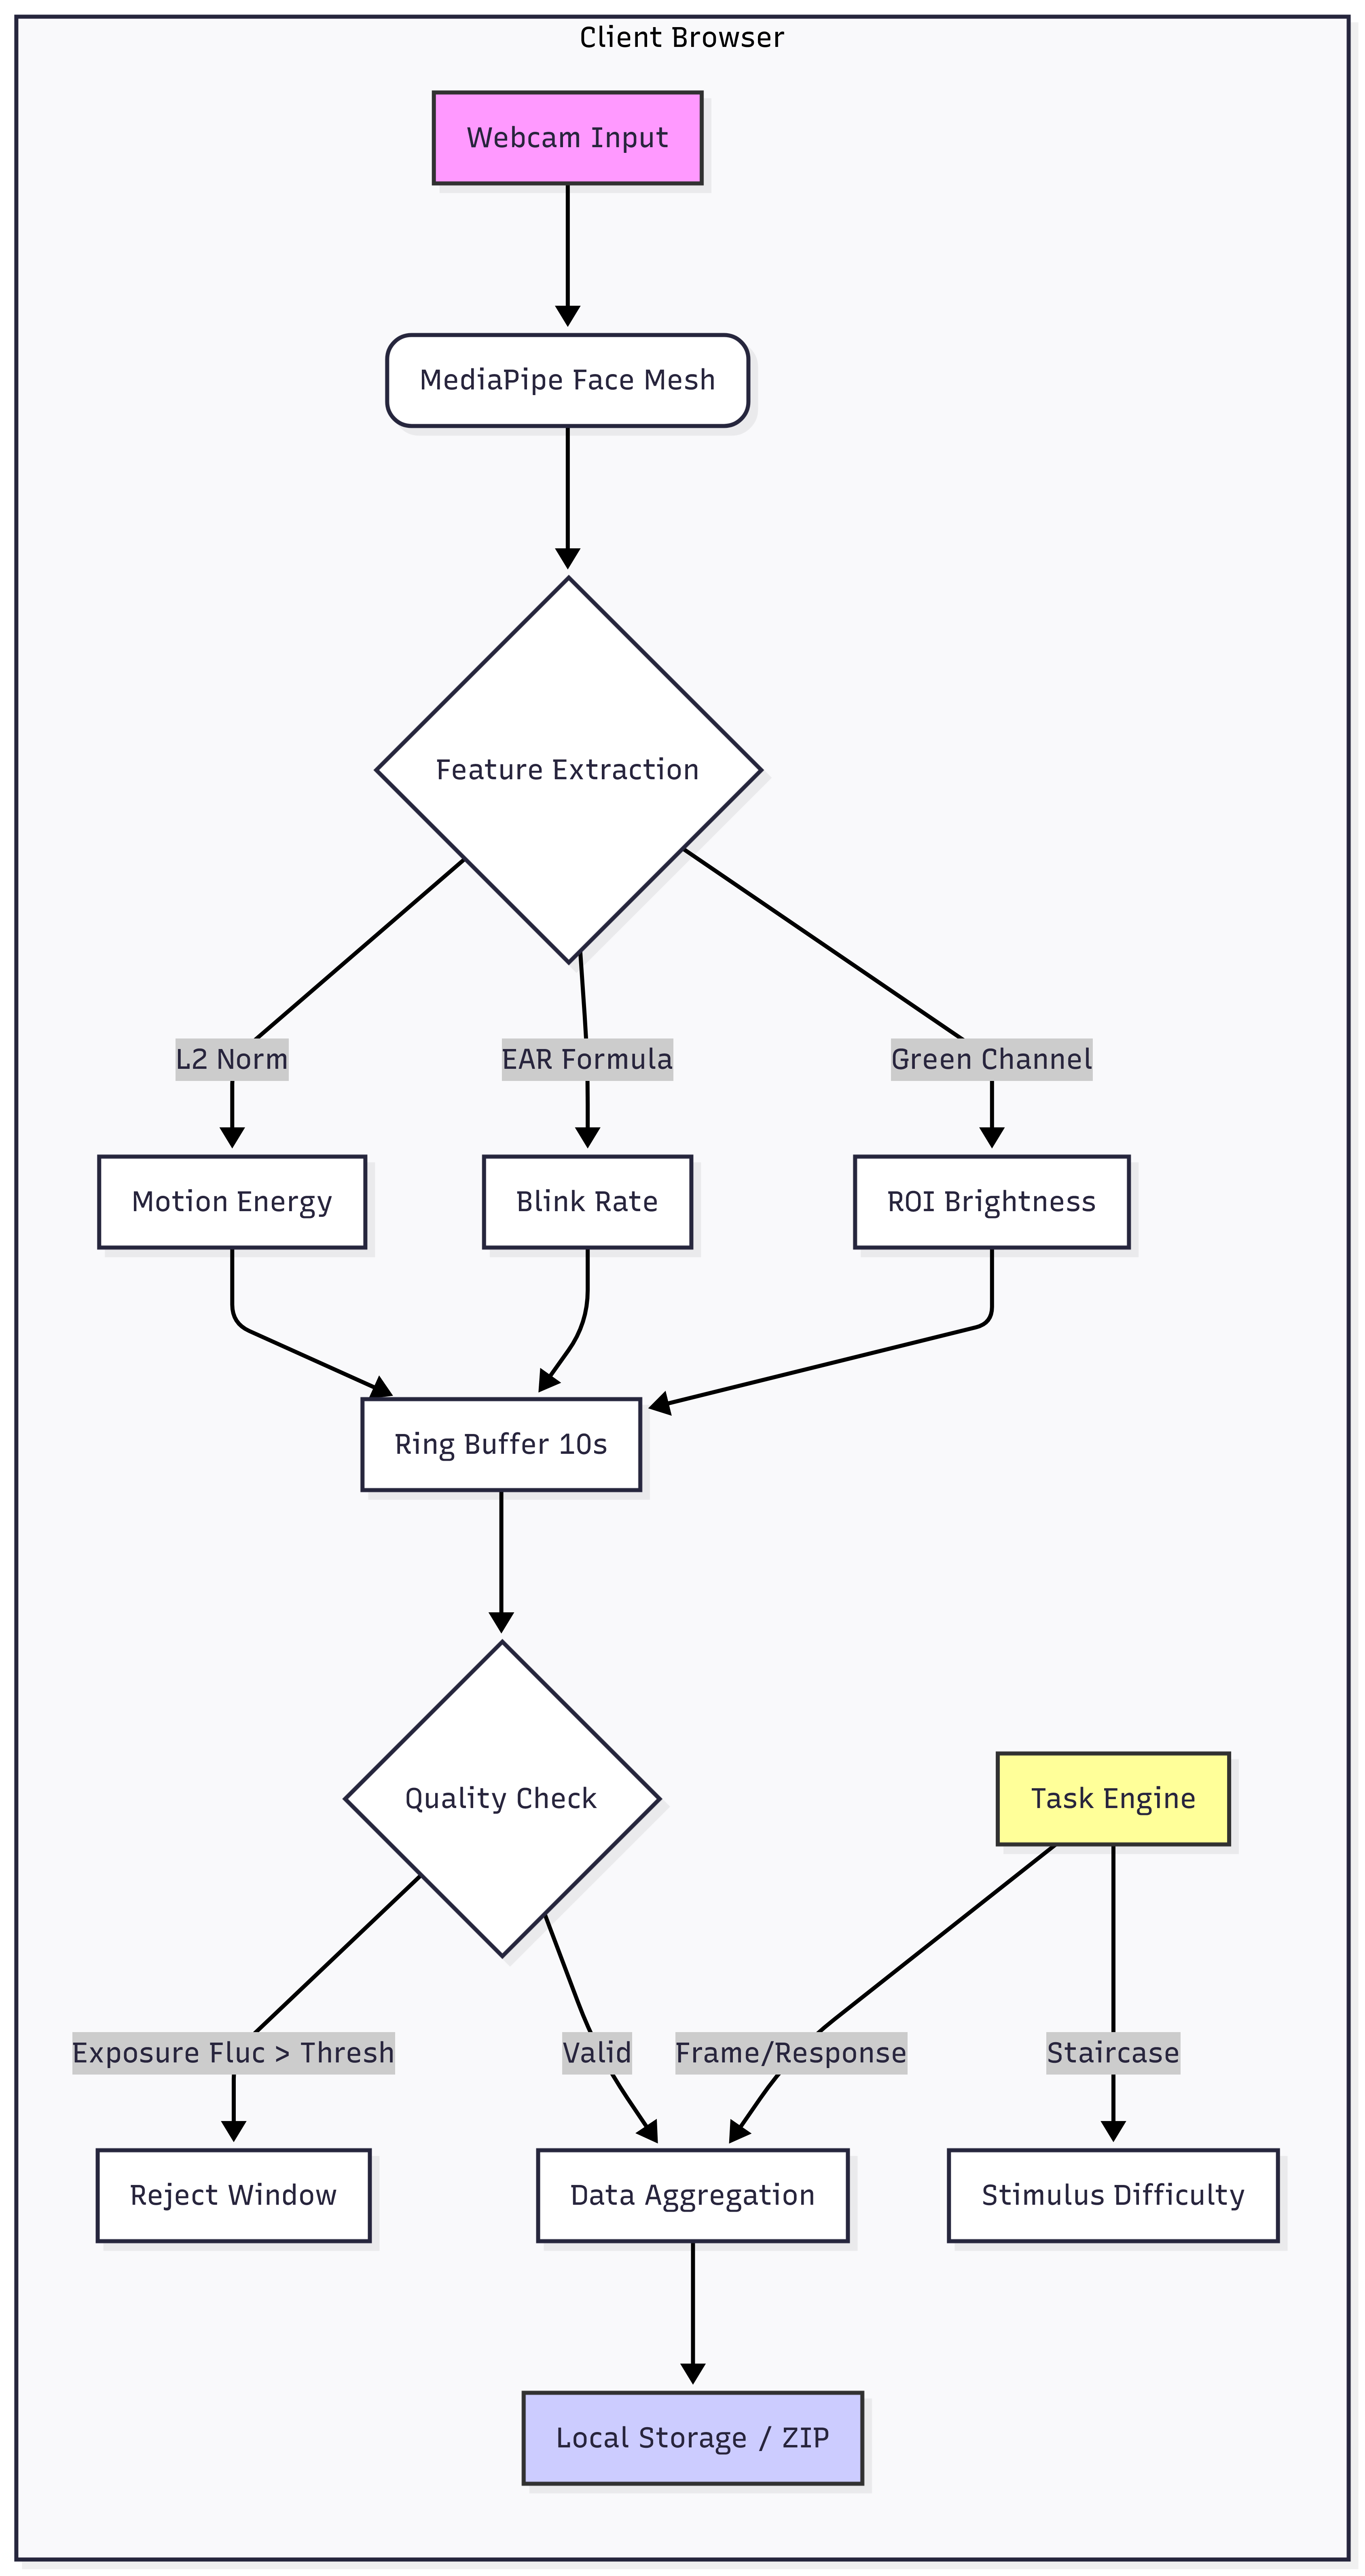
\includegraphics[width=.95\linewidth]{paper_figures/Figure1_SystemPipeline.png}
    \caption{Overview of the Camerala system architecture. The browser obtains webcam frames, extracts FaceMesh/rPPG-oriented features and quality indicators, synchronizes them with task events, and exports local logs. Under the tested implementation, only extracted features and task events are logged; raw video is neither transmitted nor stored by Camerala.}
    \label{fig:system_architecture}
\end{center}
\end{figure}

\subsection{High-Level Architecture}
The system enables a browser-based task experimental loop inside the browser sandbox (Fig. \ref{fig:system_architecture}).
The architecture consists of three coupled modules:
\begin{enumerate}
    \item \textbf{Task Engine}: Stimulus rendering, trial logic, key responses, feedback, staircase updates, and reaction-time logging.
    \item \textbf{Vision Pipeline}: Webcam ingestion, MediaPipe Face Mesh inference, rPPG-oriented ROI feature extraction, head-motion estimates, blink/EAR features, and frame-level quality indicators.
    \item \textbf{Data Manager}: Timestamp alignment, trial/frame aggregation, CSV serialization, ZIP packaging, and local persistence without raw-video storage.
\end{enumerate}

\subsection{Technical Implementation: The Vision Pipeline}
The current implementation uses MediaPipe Face Mesh as a software framework for browser-based facial landmark extraction \cite{mediapipe_framework}.
The camera stream is requested through \texttt{getUserMedia} with ideal constraints of 640$\times$480 pixels and 30 fps.
Because actual camera settings can depend on the browser and device, these constraints should be interpreted as requested settings rather than verified hardware settings.

\subsubsection{Feature Extraction Logic}
The present implementation records sensor-derived features and quality indicators rather than validated clinical or medical measurements.
Two categories are central to this paper:

\textbf{1. Head Motion Index ($M_t$)}
Head motion is approximated from the frame-to-frame displacement of a facial landmark.
Let $L^t = (x^t, y^t)$ be the normalized landmark coordinate at frame $t$.
The motion scalar is computed as:
\begin{equation}
    M_t = || L^t - L^{t-1} ||_2 .
\end{equation}
This feature is retained as a motion-related exported field for descriptive inspection of task-synchronized records.
It is not an algorithmic correction for motion artifacts in rPPG and is not used to compensate for motion-induced rPPG degradation.

\textbf{2. ROI Green-Channel Value and Brightness-Change Indicator}
The implementation samples a small forehead region around a FaceMesh landmark and records the green-channel brightness as an rPPG-oriented ROI value.
It also computes a frame-to-frame green-channel brightness-change indicator:
\begin{equation}
    B_{\Delta}(t) = | G_t - G_{t-1} | ,
\end{equation}
where $G_t$ is the downsampled frame-level green-channel average at frame $t$.
Camerala is presented as a deployment and logging architecture, not as a method for improving rPPG signal quality under motion or illumination changes.
Instead, it records motion-related and brightness-related exported fields for descriptive inspection of exported records.
The brightness-change indicator does not measure camera exposure settings, external illuminance, specific environmental events, psychological or physiological state, or rPPG accuracy.

\subsection{Technical Implementation: The Task Engine}
The experimental psychophysical probe is a two-alternative forced-choice orientation discrimination task.
Using the HTML5 Canvas API, the task engine procedurally renders oriented grating stimuli, records key responses, calculates reaction time with \texttt{performance.now()}, and updates task difficulty.
Procedural rendering avoids network-dependent stimulus loading during a trial and keeps task timing in the same browser runtime as feature logging.

\subsubsection{Timing and Synchronization}
The implementation uses the following timing strategy:
\begin{enumerate}
    \item \textbf{High-resolution timestamps}: Task events and frame features are timestamped using \texttt{performance.now()}.
    \item \textbf{Frame-loop alignment}: Feature extraction and task rendering are coordinated with the browser frame loop.
    \item \textbf{Local runtime alignment}: Task events and sensor-derived features are logged in the same browser runtime, avoiding server-side reconciliation.
\end{enumerate}

\begin{algorithm}
\caption{Camerala Task Loop (Simplified)}
\begin{algorithmic}
\STATE \textbf{Initialize} Camera, FaceMesh, Canvas
\STATE StartContinuousVisionFrameLoop()
\WHILE{Session Active}
    \STATE $Block \leftarrow$ GetCurrentBlock()
    \STATE $Context \leftarrow Block.instruction$
    \STATE ShowInstruction(Context.text)
    \FOR{trial $i = 1$ to $n$}
        \STATE $\theta \leftarrow$ SampleOrientation(\{-45$^\circ$, +45$^\circ$\})
        \STATE ShowFixation(400--600 ms)
        \STATE $t_{onset} \leftarrow$ performance.now()
        \STATE DrawOrientationStimulus($\theta$, 200 ms)
        \WHILE{No KeyPress}
            \STATE Poll F/J KeyPress
        \ENDWHILE
        \STATE $t_{response} \leftarrow$ performance.now()
        \STATE $RT \leftarrow t_{response} - t_{onset}$
        \STATE LogTaskEvent($RT$, Accuracy, Context)
        \STATE UpdateStaircase(Accuracy, relative $\pm$5\% contrast step)
        \STATE LinkTaskEventToFrameTimestamps($t_{onset}$, $t_{response}$, Context)
    \ENDFOR
\ENDWHILE
\end{algorithmic}
\end{algorithm}

\subsection{Data Management and Local-First Persistence}
The current implementation uses JSZip to export local log files as a ZIP archive.
The archive contains \texttt{metadata.json}, \texttt{trials.csv}, \texttt{features\_raw.csv}, \texttt{windows.csv}, \texttt{blocks.csv}, and \texttt{subjective.csv}.
The metadata file stores the session ID, start time, user agent, and block plan.
The user initiates the download at the end of the session.
This design avoids Camerala-side raw-video storage and avoids raw-video transmission, but it also reduces the ability to inspect image artifacts retrospectively.
For this reason, Camerala logs reproducible exported fields such as rPPG-oriented ROI green-channel values, head-motion estimates, and a frame-to-frame green-channel brightness-change indicator.

% =================================================================================
% SECTION 4: METHODOLOGY
% =================================================================================
\section{Methodology}

\subsection{Target Usage Scenario and Exploratory Deployment}
The deployment was a browser-based task experiment conducted in one laboratory setting and one home setting.
The participant sat in front of a laptop, viewed Gabor stimuli, and responded using the keyboard.
This setting should be distinguished from unconstrained daily-life physiological sensing during walking, conversation, cooking, sleep, or other ordinary activities.

To evaluate operational completion under this scenario, we conducted an exploratory longitudinal deployment with one author-participant.
The deployment consisted of 10 sessions and 600 total trials.
Each session consisted of six 10-trial blocks, with two blocks for each instructional task context (neutral instruction, negative instruction, and positive instruction), as reflected in the exported block plans.
The order of blocks was randomized by the web application.

\subsection{Participant (Autoethnography)}
The participant was the primary author.
This was a self-experimentation evaluation: no other participants were involved, no identifiable raw video was transmitted by Camerala, and the author provided informed consent for self-participation.
Because the participant was also the author and knew that the task instructions were experimentally constructed, the instruction blocks cannot be treated as validated manipulations of evaluation pressure, reward motivation, cognitive state, motivational state, or psychological state.
They are used only as exploratory task-interface contexts for demonstrating synchronized logging across task conditions.

\subsection{Hardware and Software Configuration}
Table \ref{tab:hardware_config} summarizes the hardware and software information available for the deployment.
Values that were not logged during the deployment are explicitly marked as not logged rather than inferred from the revision-time environment.

\begin{table*}[t]
\caption{Hardware and software configuration}
\label{tab:hardware_config}
\begin{center}
\small
\begin{tabular}{p{0.28\textwidth}p{0.64\textwidth}}
\toprule
\textbf{Item} & \textbf{Reported value} \\
\midrule
Laptop/PC model & mouse Computer G-Tune P517G60ZO21CNHWT \\
CPU & Intel Core i7-13620H, 10 cores (P6+E4), 16 threads \\
GPU & NVIDIA GeForce RTX 5060 Laptop GPU \\
RAM & 32 GB \\
Storage & 1 TB SSD \\
Operating system & Windows 11 Home 64-bit; exact deployment-time build not logged \\
Display & 15.6-inch display, 2560$\times$1440 pixels, 165 Hz \\
Browsers used & Mozilla Firefox and Google Chrome \\
Browser versions & Firefox user-agent was available when recorded in exported metadata; exact Chrome deployment-time version was not systematically logged \\
Webcam type & Built-in laptop webcam \\
Webcam model & Exact internal webcam model not logged \\
Camera capture API & Browser \texttt{getUserMedia} API \\
Requested camera constraints & Ideal 640$\times$480 pixels, ideal 30 fps \\
Actual camera resolution & Browser/device-negotiated; not programmatically logged as a verified deployment-time value \\
Actual camera frame rate & Browser/device-negotiated; not programmatically logged as a verified camera frame rate \\
Screen brightness & Fixed during the deployment; exact percentage not logged \\
Auto-exposure & Device/browser default behavior; not manually constrained and exact state not programmatically logged \\
Auto-white-balance & Device/browser default behavior; not manually constrained and exact state not programmatically logged \\
\bottomrule
\end{tabular}
\end{center}
\end{table*}

\subsection{Deployment Environment and Lighting Conditions}
The deployment was conducted during daytime in an indoor university laboratory/research room and an indoor private home room under general artificial room lighting.
Both rooms had windows, but curtains were closed during the sessions.
Direct natural light was not used as the primary illumination source in either context.
The built-in laptop display brightness was fixed across sessions.
Because the deployment used camera-derived setup checks rather than external light-meter measurements, this paper reports brightness ranges only as author-confirmed setup/check information.
The camera-derived brightness range observed during setup/checks was 105--114 in the laboratory setting and 102--111 in the home setting.
Table \ref{tab:environment_config} summarizes the deployment environment and lighting conditions.

\begin{table*}[t]
\caption{Deployment environment and lighting conditions}
\label{tab:environment_config}
\begin{center}
\small
\begin{tabular}{p{0.24\textwidth}p{0.32\textwidth}p{0.32\textwidth}}
\toprule
\textbf{Item} & \textbf{Laboratory} & \textbf{Home} \\
\midrule
Room type & Indoor university laboratory/research room & Indoor private home room \\
Time of day & Daytime & Daytime \\
Primary lighting & General indoor artificial lighting & General indoor artificial lighting \\
Window presence & Windows present & Windows present \\
Curtain/blind condition & Curtains present and closed & Curtains present and closed \\
Natural light contribution & Direct natural light was not used as the primary illumination source & Direct natural light was not used as the primary illumination source \\
Camera-derived brightness range observed during setup/checks & 105--114 & 102--111 \\
External light-meter measurement & \multicolumn{2}{p{0.64\textwidth}}{External light-meter values were not used; the reported ranges are camera-derived setup/check information, not lux measurements.} \\
Screen brightness & \multicolumn{2}{p{0.64\textwidth}}{Fixed across sessions using the built-in laptop display setting.} \\
Task display & \multicolumn{2}{p{0.64\textwidth}}{Stimuli were presented on the built-in laptop display. Screen luminance was part of the tested configuration rather than an independently manipulated factor.} \\
Window aggregation & \multicolumn{2}{p{0.64\textwidth}}{Exported window-level features used 10-s windows with 5-s overlap.} \\
Brightness-change indicator aggregation & \multicolumn{2}{p{0.64\textwidth}}{The frame-to-frame green-channel brightness-change indicator was summarized in 10-s windows with 5-s overlap.} \\
Clouds/screen flicker/power cycles & \multicolumn{2}{p{0.64\textwidth}}{Not treated as observed experimental events; possible brightness variation was handled only as camera-image-derived record variation.} \\
\bottomrule
\end{tabular}
\end{center}
\end{table*}

\subsection{Experimental Procedure and Instructional Task Contexts}
Each session began with a pre-session capture check for basic camera conditions, including approximate camera-derived brightness and pose, before the camera feed was hidden to reduce distraction.
The task included negative, neutral, and positive instruction contexts as exploratory task-interface conditions.
These contexts were used to demonstrate that Camerala can present different instruction frames while recording synchronized behavioral and face-derived records.
The labels ``negative'' and ``positive'' refer only to instruction labels used in the task interface.
Because the participant was the author and knew that the instructions were experimentally constructed, these contexts are not treated as validated manipulations of evaluation pressure, reward motivation, cognitive state, or motivational state.

\subsection{Psychophysical Task}
The task was a two-alternative forced-choice orientation discrimination task using procedurally rendered Gabor stimuli.
Each trial began with a randomized fixation period of 400--600 ms, followed by a Gabor stimulus oriented at either $+45^\circ$ or $-45^\circ$ for 200 ms.
The participant responded using the F/J keys: the F key corresponded to $-45^\circ$, and the J key corresponded to $+45^\circ$.
The application recorded stimulus onset, response key, reaction time, correctness, and task difficulty together with frame-level sensor-derived features.
To maintain adaptive task difficulty, the implementation used a standard 1-up 1-down staircase procedure on stimulus contrast.
Stimulus contrast was adjusted by relative $\pm 5\%$ steps according to the previous response.
These task parameters are reported for reproducibility; the instruction blocks are not interpreted as validated cognitive or motivational manipulations.

\subsection{Dependent Measures and Pre-processing}
All exported logs were processed sequentially.
The primary behavioral measure was reaction time (RT), with an operational analysis range of 100--1500 ms.
The primary sensor-derived measures were rPPG-oriented ROI green-channel values, head-motion estimates, and the frame-to-frame green-channel brightness-change indicator.
Behavioral trials were retained when reaction times fell within 100--1500 ms.
Camerala used MediaPipe FaceMesh to obtain facial landmarks in the browser.
Frame records forwarded from the FaceMesh callback were synchronized with task events during active sessions.
The feature extractor defines a binary landmark-availability flag, \texttt{quality}, where 1 indicates that FaceMesh landmarks were returned and 0 indicates that no landmarks were returned.
In the current runtime, however, the camera manager forwards results to the logging callback only when FaceMesh landmarks are returned; therefore, the saved frame records in this deployment represent landmark-returned exported frames.
For each exported 10-s window, \texttt{mean\_quality} was computed as the mean of the \texttt{quality} flag over the exported frame records in that window.
Thus, \texttt{mean\_quality} describes landmark availability within exported frame/window records and not face-detection availability across all camera frames.
This value is not a continuous MediaPipe confidence score, an indicator of rPPG measurement quality, or evidence of physiological measurement accuracy.
The FaceMesh \texttt{minDetectionConfidence} and \texttt{minTrackingConfidence} parameters were both set to 0.5 as implementation settings.
They were not used as post-hoc analysis thresholds.

% =================================================================================
% SECTION 5: RESULTS
% =================================================================================
\section{Results}

The results are reported descriptively as sensor-derived observations under the tested configuration.
The deployment completed all 10 planned sessions and 600 trials in total.
After applying the reaction-time criterion of 100--1500 ms, 541/600 trials were retained for descriptive analysis.
The retained trials were 256/300 in the laboratory setting and 285/300 in the home setting.
All 299 exported windows had \texttt{mean\_quality} = 1.0 and therefore satisfied the operational landmark-availability criterion of \texttt{mean\_quality} $\geq$ 0.8; no window was excluded by this criterion.
These results describe the available analyzed trials and exported windows under the tested configuration and do not demonstrate general feasibility across devices, users, or environments.

\subsection{Task and Exported Feature Summaries}
Table \ref{tab:data_quality} summarizes task-level and exported feature summaries in the laboratory and home contexts.
After RT exclusion, mean RT was 721.1 $\pm$ 257.7 ms in the laboratory setting and 676.5 $\pm$ 249.5 ms in the home setting.
Accuracy was 85.5\% and 82.1\%, respectively.
Window-level exported records showed descriptive differences in ROI green-channel values, motion estimates, and the brightness-change indicator between settings.
Because lighting, screen light, posture, camera geometry, task timing, and participant state were not independently controlled, these differences are reported only as deployment-context differences in exported records.

\begin{table*}[t]
\centering
\caption{Descriptive task and exported feature summaries after reaction-time exclusion.}
\label{tab:data_quality}
\footnotesize
\begin{tabular}{@{}p{0.30\textwidth}p{0.18\textwidth}p{0.18\textwidth}p{0.24\textwidth}@{}}
\toprule
\textbf{Metric} & \textbf{Laboratory} & \textbf{Home} & \textbf{Notes} \\
\midrule
Retained trials after RT exclusion & 256/300 (85.3\%) & 285/300 (95.0\%) & Trial-level; RT 100--1500 ms \\
Mean RT after RT exclusion & 721.1 $\pm$ 257.7 ms & 676.5 $\pm$ 249.5 ms & Trial-level retained trials \\
Accuracy after RT exclusion & 85.5\% & 82.1\% & Trial-level retained trials \\
rPPG-oriented ROI green-channel value & 46.69 $\pm$ 6.80 & 34.32 $\pm$ 2.72 & Window-level; windows.csv \\
Motion estimate & 0.0011 $\pm$ 0.0005 & 0.0010 $\pm$ 0.0004 & Window-level; windows.csv \\
Frame-to-frame green-channel brightness-change indicator & 0.0504 $\pm$ 0.0509 & 0.0707 $\pm$ 0.0337 & Window-level; windows.csv \\
\bottomrule
\end{tabular}
\end{table*}

\subsection{Task-Event and Sensor-Derived Observations}
To address RQ2, we compared descriptive task-synchronized records between the laboratory and home contexts.
The exported records showed differences in rPPG-oriented ROI green-channel values, motion estimates, and the frame-to-frame green-channel brightness-change indicator.
Because lighting, screen light, posture, camera geometry, task timing, and participant state were not independently controlled, these differences are reported only as deployment-context differences in exported records.
They should not be interpreted as evidence that the instruction blocks induced psychological, cognitive, motivational, or physiological effects.
Motion estimates are reported as exported face-derived records for descriptive comparison between the laboratory and home contexts.
They are not interpreted as evidence of motion handling or correction of rPPG degradation.

The instruction contexts were used only as task-interface contexts in the deployment.
We do not report them as evidence that evaluation pressure, reward motivation, cognitive effects, or motivational effects were induced.
Descriptive values are reported by instruction context only to document that the logging pipeline operated across different task-interface contexts.
In the laboratory context, the negative instruction block showed a lower mean RT than the neutral block in this dataset.
In the home context, the mean RT values across instruction blocks were closer together.
Because the deployment used one author-participant and did not isolate instruction effects from environment, lighting, screen light, posture, camera geometry, or measurement-pipeline factors, these RT patterns are reported only as descriptive task-event observations.

\subsection{rPPG-Oriented ROI Estimates}
The exported data include rPPG-oriented ROI brightness values and related quality indicators, but no ECG or contact PPG reference was collected.
Therefore, this paper does not interpret ROI-derived or block-level summaries as validated heart-rate changes.
The appropriate interpretation is that the tested deployment yielded face-derived and sensor-derived exported records whose values differed descriptively between the tested laboratory and home contexts.

% =================================================================================
% SECTION 6: DISCUSSION
% =================================================================================
\section{Discussion}

The main implication of this deployment is not that home or laboratory settings affect camera-based physiological records; this is a known limitation of video-based sensing.
Instead, the deployment illustrates design requirements for a local-first, browser-native logging architecture for remote psychological and psychophysiological task experiments.
In particular, when raw facial video is not retained, the system must preserve task-event timestamps, exported face-derived records, operational landmark-availability checks, motion and brightness-change records, and sufficient hardware/environment metadata to support cautious post-hoc interpretation.
Under the tested configuration, Camerala completed the planned task procedure and exported task-synchronized records for descriptive analysis.
However, the laboratory/home differences should be interpreted as mixed deployment-context differences rather than psychological, cognitive, motivational, or physiological effects.
Future versions should include pre-session camera and lighting checks, explicit operational criteria, reference physiological sensors, multiple participants, multiple devices, and controlled lighting, posture, and camera conditions.

Camerala's useful system property is integration: task timing, frame-level feature extraction, quality indicators, and local export are handled in one client-side workflow.
This can reduce raw-video handling and server-side timestamp reconciliation, but it also removes the possibility of visually inspecting many artifacts after data collection.
The trade-off makes quality-aware logging important.
The relevant indicators include landmark availability, rPPG-oriented ROI values, head-motion estimates, and camera-image-derived brightness-change records; these values can support pre-session checks and descriptive inspection, but they are not proof that rPPG estimates are accurate or that motion-induced rPPG degradation has been corrected.

The laboratory/home differences observed in this deployment should be interpreted as mixed deployment-context differences that may reflect environmental conditions, screen light, posture, camera geometry, the measurement pipeline, task timing, participant state, or their mixture.
The study was not designed to isolate psychological or physiological state changes from these factors, and it cannot validate the psychological effectiveness of the negative or positive instruction contexts.
Future deployments should therefore incorporate task-event/frame-record timestamp alignment, operational landmark-availability criteria, documented hardware/browser/camera settings, explicit reporting of camera constraints and actual camera settings, fixed screen-brightness settings, pre-session camera/lighting checks, landmark-availability warnings, motion and camera-derived brightness-change records, environment reporting, and specified quality-aware analysis rules.
If privacy-sensitive raw video is not stored, these safeguards become more important because many artifacts cannot be retrospectively inspected from images; for studies that aim to make claims about physiological responses, a reference physiological sensor and a multi-participant design are necessary.

\subsection{Limitations}
This exploratory N=1 author-participant deployment used one primary laptop/camera configuration, no ECG or contact PPG reference, and no comparison with existing experiment runtimes, browser rPPG tools, or cloud APIs.
It did not test multiple participants, devices, or home environments, and it did not experimentally separate lighting, screen light, posture, camera placement, task timing, participant state, and task context.
The implementation does not correct motion-induced rPPG degradation, and the logs do not store continuous confidence values for all frames; therefore, failed landmark-detection frames and overall tracking-success rates cannot be recovered.
Future work should use reference physiological sensors, controlled posture/camera conditions, predefined artifact-handling rules, and continuous confidence logging with specified operational thresholds.
The study does not claim clinical or medical accuracy, general deployability, general feasibility, or validated cognitive, motivational, psychological, or physiological effects; it presents an implementation example of browser-native, task-aligned, local-first feature logging under limited laboratory and home conditions.

\section{Conclusion}
We presented Camerala, a browser-native, local-first implementation example that integrates psychophysical task execution, face-derived feature extraction, task-event/frame-record timestamp alignment, operational landmark-availability checking, and local CSV/ZIP persistence without raw facial video retention.
In a limited 10-session N=1 author-participant deployment across one laboratory setting and one home setting, Camerala completed 600 trials, and 541/600 trials remained after the specified reaction-time criterion.
The deployment produced synchronized behavioral logs and face-derived and sensor-derived records with descriptive deployment-context differences between the tested environments.
These observations should not be interpreted as evidence of general deployability or physiological/cognitive effects; instead, they highlight design safeguards needed for future local-first physiological feature logging in home-based psychophysical experiments.

\section*{Declarations}
\textbf{Data availability.}
The dataset cannot be made publicly available because it contains privacy-sensitive face-derived records from a domestic deployment context.

\textbf{CRediT authorship contribution statement.}
\textbf{Kotaro Furukawa}: Conceptualization, Methodology, Software, Investigation, Formal analysis, Writing - original draft.

\textbf{Declaration of competing interest.}
The author declares no competing interests.

\textbf{Funding.}
This work was supported by the College of Transdisciplinary Sciences for Innovation, Kanazawa University.

{\footnotesize
\begin{thebibliography}{99}
\footnotesize\baselineskip=9pt\setlength{\itemsep}{0pt}\setlength{\parsep}{0pt}

\bibitem{verkruysse2008}
Wim Verkruysse, Lars~O. Svaasand, and J. Stuart Nelson.
\newblock Remote plethysmographic imaging using ambient light.
\newblock {\em Optics Express}, 16(26):21434--21445, 2008.

\bibitem{poh_ica}
Ming-Zher Poh, Daniel~J. McDuff, and Rosalind~W. Picard.
\newblock Non-contact, automated cardiac pulse measurements using video imaging and blind source separation.
\newblock {\em Optics Express}, 18(10):10762--10774, 2010.

\bibitem{deepphys}
Weixuan Chen and Daniel McDuff.
\newblock Deepphys: Video-based physiological measurement using convolutional attention networks.
\newblock In {\em Proceedings of the European Conference on Computer Vision (ECCV)}, pages 349--365, 2018.

\bibitem{ayesha_web_vital}
A.~H. Ayesha, D. Qiao, and F. Zulkernine.
\newblock A web application for experimenting and validating remote measurement of vital signs.
\newblock In {\em Information Integration and Web Intelligence (iiWAS 2022)}, Lecture Notes in Computer Science, vol. 13635, pages 237--251, 2022.
\newblock doi:10.1007/978-3-031-21047-1\_21.

\bibitem{labvanced_rppg}
LabVanced.
\newblock Remote heart rate detection / rPPG.
\newblock \url{https://www.labvanced.com/content/technology/en/remote-heart-rate-detection-rPPG/}, accessed July 5, 2026.

\bibitem{facephys_demo}
K. Wang.
\newblock FacePhys-Demo: Browser-based rPPG monitor with local inference.
\newblock \url{https://github.com/KegangWangCCNU/FacePhys-Demo}, accessed July 5, 2026.

\bibitem{rhythmedge}
Z. Hasan, E. Dey, S.~R. Ramamurthy, N. Roy, and A. Misra.
\newblock Demo: RhythmEdge: Enabling contactless heart rate estimation on the edge.
\newblock In {\em 2022 IEEE International Conference on Smart Computing (SMARTCOMP)}, pages 177--179, 2022.

\bibitem{gupta_privacy}
D. Gupta and A. Etemad.
\newblock Privacy-preserving remote heart rate estimation from facial videos.
\newblock In {\em 2023 IEEE International Conference on Systems, Man, and Cybernetics (SMC)}, pages 706--712, 2023.
\newblock doi:10.1109/SMC53992.2023.10394350.

\bibitem{di_lernia_rppg_wild}
D. Di~Lernia, G. Finotti, M. Tsakiris, G. Riva, and M. Naber.
\newblock Remote photoplethysmography (rPPG) in the wild: Remote heart rate imaging via online webcams.
\newblock {\em Behavior Research Methods}, 56:6904--6914, 2024.
\newblock doi:10.3758/s13428-024-02398-0.

\bibitem{jspsych_joss}
J.~R. de Leeuw, R.~A. Gilbert, and B. Luchterhandt.
\newblock jsPsych: Enabling an open-source collaborative ecosystem of behavioral experiments.
\newblock {\em Journal of Open Source Software}, 8(85):5351, 2023.
\newblock doi:10.21105/joss.05351.

\bibitem{psychopy2}
J.~W. Peirce, J.~R. Gray, S. Simpson, M. MacAskill, R. Hoechenberger, H. Sogo, E. Kastman, and J.~K. Lindelov.
\newblock PsychoPy2: Experiments in behavior made easy.
\newblock {\em Behavior Research Methods}, 51:195--203, 2019.
\newblock doi:10.3758/s13428-018-01193-y.

\bibitem{mediapipe_framework}
Google AI Edge.
\newblock MediaPipe Face Landmarker.
\newblock \url{https://ai.google.dev/edge/mediapipe/solutions/vision/face_landmarker}, accessed July 5, 2026.

\end{thebibliography}
}

\end{document}
